As illustrated in Figure \ref{fig:PV_system_configuration_cell_module_array}, the building
blocks of a PV array are the modules, which consist of a number of PV cells connected in
series. These modules can be connected in series to form a module string, and several
module strings connected in parallel form a PV array. The array links to a solar inverter,
which transforms the produced direct current (DC) power into alternating current (AC)
power for load consumption and connection to the electrical grid. A PV plant is composed
of one or multiple PV arrays. Hence, the PV cells, the basic units of PV modules, are the
starting points for performance modeling of entire PV systems and plants \cite[p. 305f]{Ma2014_1}.
The mathematical models for a single cell can be extended to arrays \cite{Ma2014_2, Tian2012},
and therefore to entire PV plants.
The general approach to assessing the electrical performance of a PV cell is based on the
ability to analytically describe its current-voltage characteristic by modeling it with an
equivalent electrical circuit that includes some nonlinear components \cite[p. 1359]{LoBrano}.
These circuits are composed of a current source, one or two antiparallel diodes (D),
with or without an internal series resistance \(R_{\text{s}}\) (\si{\ohm}) and a shunt
resistance \(R_{\text{sh}}\) (\si{\ohm}). A graphical visualization of the equivalent
circuit models is shown in Figure
\ref{fig:Overview_equivalent_circuit_models}. The authors of \cite{Ma2014_1}
have conducted a comprehensive literature review on PV cell mathematical
models, whose governing equations can be summarized as follows:

\begin{itemize}
    \item Ideal model:
    \begin{align}
        I &= I_{\text{L}} - I_{\text{D}} = I_{\text{L}} - I_{\text{0}} \Bigl[ \exp \Bigl( \frac{V}{nT} \Bigr) - 1 \Bigr]
        \label{eq:Three_parameter_model}
    \intertext{\item One-diode model with \(R_{s}\):}
        I &= I_{\text{L}} - I_{\text{D}} = I_{\text{L}} - I_{\text{0}} \Bigl[ \exp \Bigl( \frac{V + IR_{\text{s}}}{nT} \Bigr) - 1 \Bigr]
        \label{eq:Four_parameter_model}
    \intertext{\item One-diode model with \(R_{\text{s}}\) and \(R_{\text{sh}}\):}
        I &= I_{\text{L}} - I_{\text{D}} = I_{\text{L}} - I_{\text{0}} \Bigl[ \exp \Bigl( \frac{V + IR_{\text{s}}}{nT} \Bigr) - 1 \Bigr] - \frac{V + IR_{\text{s}}}{R_{\text{sh}}}
        \label{eq:Five_parameter_model}
    \intertext{\item Two-diode model:}
        I &= I_{\text{L}} - I_{\text{D}_{1}} - I_{\text{D}_{2}} \nonumber \\
          &= I_{\text{L}} - I_{0,1} \Bigl[ \exp \Bigl( \frac{V + IR_{\text{s}}}{n_1T} \Bigr) - 1 \Bigr] - I_{0,2} \Bigl[ \exp \Bigl( \frac{V + IR_{\text{s}}}{n_2T} \Bigr) - 1 \Bigr] - \frac{V + IR_{\text{s}}}{R_{\text{sh}}}
          \label{eq:Seven_parameter_model}    
    \end{align}
\end{itemize}

\noindent
Here, \(I_{\text{L}}\) is the light-generated current (\si{\ampere}) , \(I_{0(,i)}\) is the reverse saturation
current (\si{\ampere}), \(n_{(i)}\) is the diode ideality factor and \(T\) is the cell temperature (\si{\kelvin}).
The unknowns in the above equations are the current \(I\) and voltage \(V\), whereas the rest
denote model parameters that are either constant or depend on the operating conditions
discussed in Section \ref{sec:Operating_conditions}. Thus, the models in Equations
\ref{eq:Three_parameter_model}, \ref{eq:Four_parameter_model}, \ref{eq:Five_parameter_model},
and \ref{eq:Seven_parameter_model} are also referred to as three-, four-, five-,
and seven-parameter models, respectively. The denominator in the exponential terms
is often written as the diode thermal voltage \(V_{T} = nkT/q\) where \(k\) is
Boltzmann's constant, \(T\) is the cell temperature and \(q\) is the charge
of an electron. Both \(nT\) and \(V_{T}\) can be used as representations
of the thermal voltage in the diode equations as \(q\) and \(k\) are constants.
The results of their literature review indicate that the ideal model, which
neglects internal resistance effects, is not suitable for modeling the PV cell
behavior \cite{Mazhari2006}. Furthermore, compared with the five-parameter model,
the four-parameter model does not satisfactorily reflect the effect of high
temperature on the current \cite{Celik2007, Karamirad2013}, leading to less
accurate predictions. Nevertheless, these models have their justification,
as the authors of \cite{Dolora2015} show in their comparative study.
The two-diode model accounts for the reality that the reverse saturation
current is the result of a linear superposition of charge diffusion and
recombination in the space-charge region \cite{Gow1999}, which is reflected
by the two diodes in the model. It can achieve greater accuracy than the
five-parameter model, particularly at low irradiance levels and during
partial shading conditions \cite{Ishaque2011}. The major drawback of the
two-diode model is the high number of parameters, which increase the
computational burden and result in relatively long computation times
\cite{Ishaque2011_2, Ishaque2011_1}.
Despite the higher accuracy of the two-diode model, the five-parameter model
offers a good balance between accuracy and computational efficiency.
This model effectively captures the key electrical
characteristics of a PV cell under various operating conditions while keeping
the complexity manageable for practical applications. Therefore, the
five-parameter model is widely used in PV system simulations and is selected
for this thesis.

\begin{figure}
    \centering
    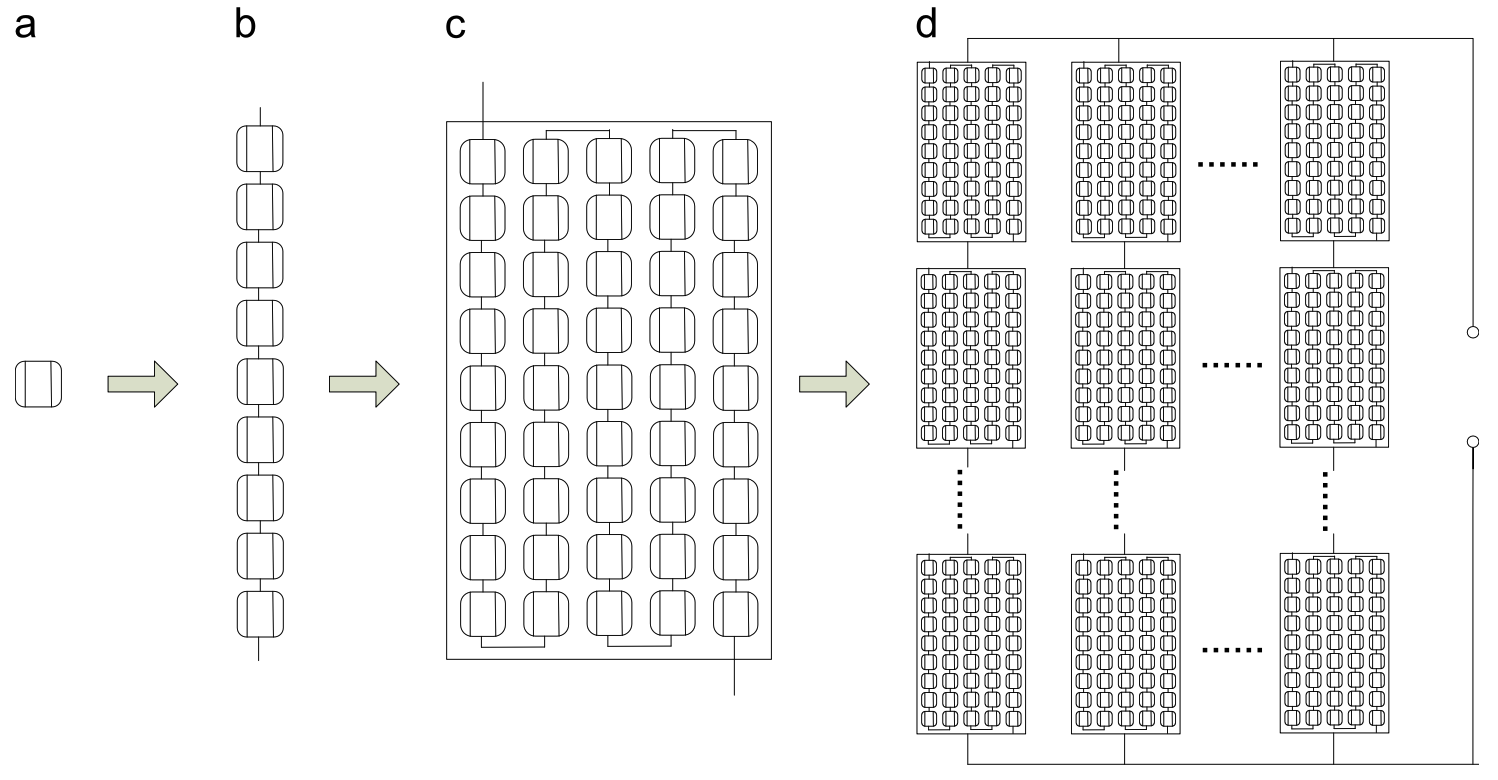
\includegraphics[scale=0.28]{PV_system_configuration_cell_module_array.png}
    \caption{\small Physical configuration of (a) PV cell, (b) cell series string, (c) module
             and (d) PV array \cite{Ma2014_1}.}
    \label{fig:PV_system_configuration_cell_module_array}
\end{figure}

\begin{figure}
    \centering
    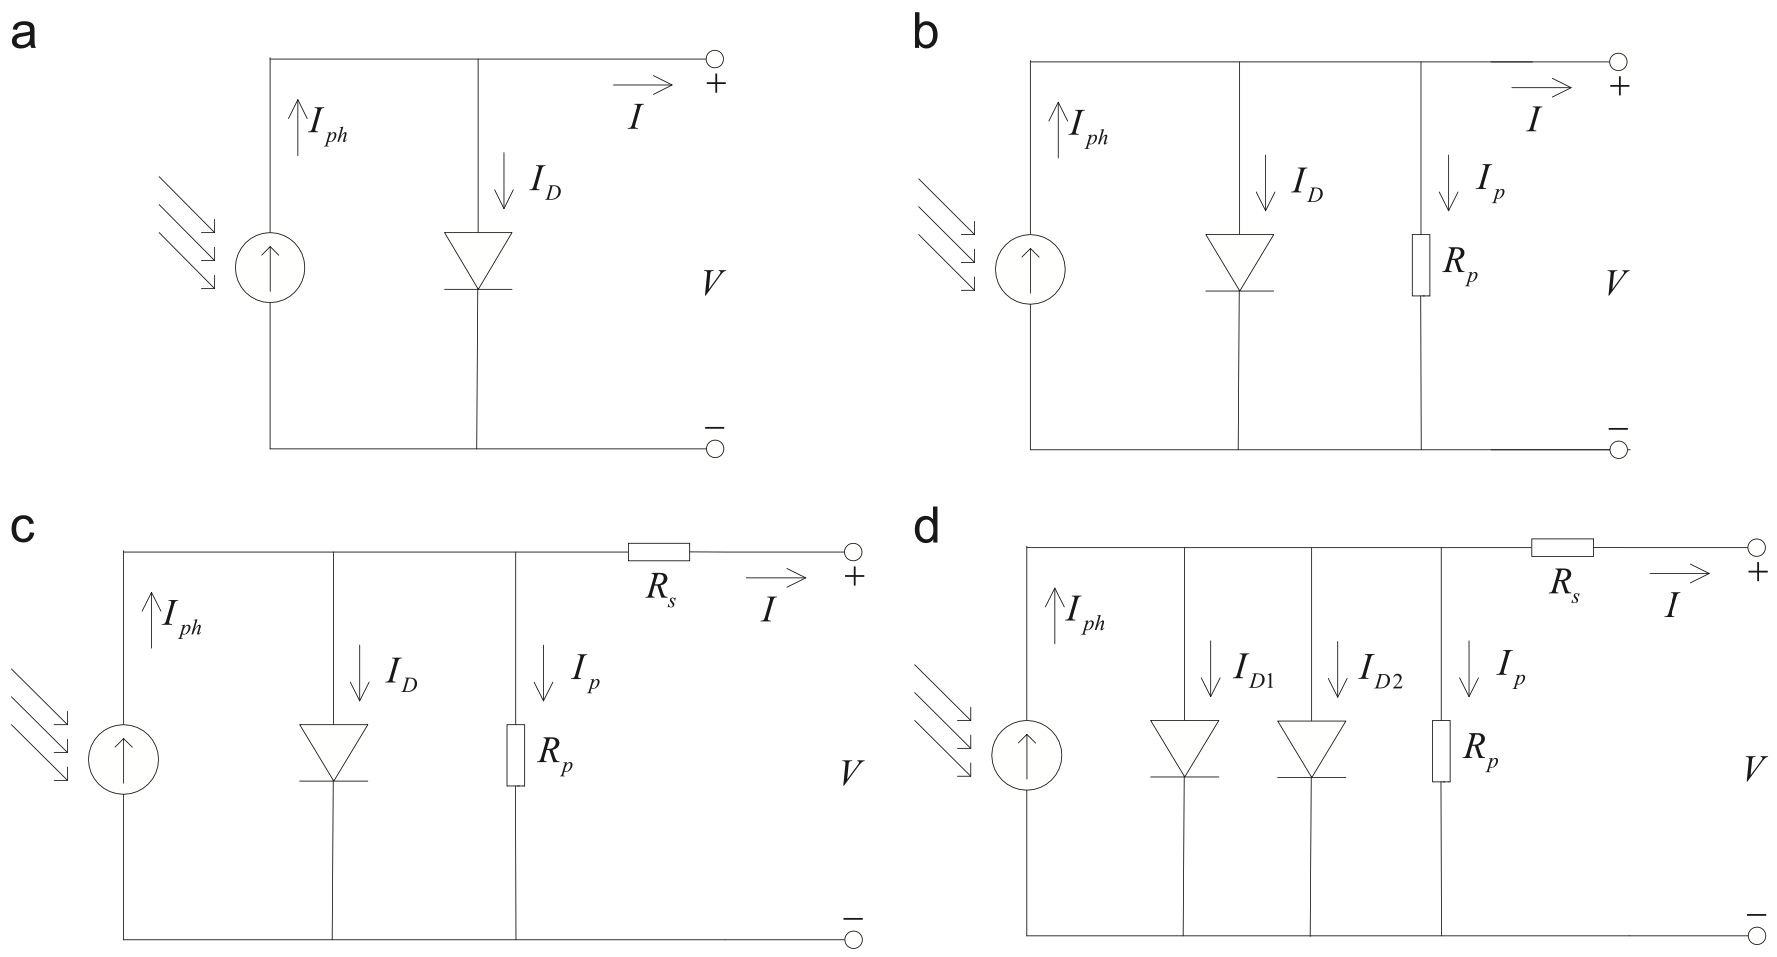
\includegraphics[scale=0.243]{Overview_equivalent_circuit_models.png}
    \caption{\small Equivalent PV cell electrical circuits: (a) ideal model,
        (b) one-diode with \(R_{\text{s}}\), (c) one-diode with \(R_{\text{s}} \text{ and } R_{\text{sh}}\),
        and (d) two-diode model \cite{Ma2014_1}.}
        \label{fig:Overview_equivalent_circuit_models}
\end{figure}
